\documentclass[12pt]{article}
\usepackage{graphicx}
\begin{document}
\begin{center}
  {\large\bf Detector Resolution}
\end{center}
\vskip0.2in
\begin{enumerate}
\item {\it Measurement Uncertainties} 
The {\it Central Limit Theorm} tells us  that 
the distribution of the sum (or average) of a large number of independent, identically 
distributed measurements will be approximately normal, regardless of the underlying distribution
(subject to the condition that mean and variance of the underlying distribution are not infinite).
We'll see how this works for the simplest pdf, a random variable $x$ uniformly distributed:
$$
f(x) = 
\left\{ \begin{array}{rl}
 \frac{1}{b-a} &\mbox{ if $a \le x \le b$} \\
  0 &\mbox{ otherwise}
       \end{array} 
\right.
$$ 
\begin{enumerate}
\item Use the definitions of mean and sigma to
calculate the mean $\mu$ and the variance $\sigma^2$ of the distribution.
\item Let $a=0$ and $b=1$. Using your favorite random number generator, generate 1000 random numbers.  Calculate the
  mean and sigma of the numbers you have generated
  and verify that the results are consistent with your result from  part (a). 
\item Make a histogram  with 100 bins where the lower edge of the first bin is at $x=0$ and the upper
edge of the last is at $x=1$.  Fill your histogram with the random numbers you generated in part (b).  
\item Now suppose you make an ensemble of 1000 pseudoexperiments where each pseduoexperiment consists of $N$
uniformly distributed random numbers.  For each pseudoexperiment, define the measurement $S$ to be
$$
S \equiv \frac{1}{N} \sum_1^N x_i
$$
Make histograms of $S$ with the same $x-$axis as in part (c) for the cases $N=2$, $N=5$
and $N=10$.  Determine the mean and the $\sigma$ of the distributions displayed in
these histograms.  In each case, compare the
$\sigma$ you obtain to what you would predict if you assumed the experiments followed a normal distribution.
\end{enumerate}
\item {\it Silicon Detector Position Resolution:  Analytic Calculation}
In this problem and the next we will study
how the position resolution of a detector
depends upon the properties of that detector.  
For our example, we will consider a silicon micro-strip detector.
%\begin{figure}[h]
%\begin{center}
%\includegraphics[width=3.0in]{figs_ps/Silicon_Detector.pdf}
%\end{center}
%\end{figure}
We will describe our
detector as a plane segmented into strips, each of width $\ell$.  When
a track passes through the plane, it deposits energy in the detector
and that energy is collected using charge sensitive amplifiers (one per
strip).  You many assume that the incident track is normal to the 
silicon plane.  Looking down on the strip detector (so that the incident
tracks are traveling into the page), the
detector looks like this:
\vskip0.05in
\begin{figure}[h]
\begin{center}
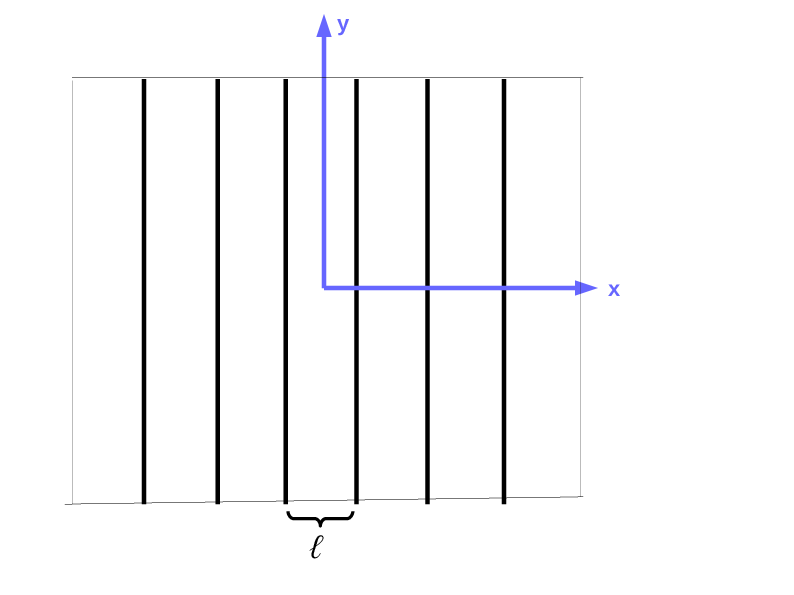
\includegraphics[width=4.0in]{strips.png}
\end{center}
\end{figure}
The position $x=0, y=0$ is taken to be the center of the middle
strip.
\begin{enumerate}
\item Suppose all the energy is deposited in a single strip (the strip the
track passes through).  Find an expression for the position resolution
of the detector as a function of $\ell$. The position resolution is defined
to be $\sigma_x = \sqrt{var[(x_{meas}-x_{true})]}$ where $x_{true}$ is the 
position where the track actually hit the detector.  Because we only
know which strip is hit, in this example 
$x_{meas}$ is the center of the strip that is hit. 
\item Suppose that 
the charge deposited in our detector spreads out due
to physical effects such as diffusion. It is possible for more than
one strip to register a signal.  Assume in this part that our electronics
is binary (ie registers a 1 if the deposited energy on the
strip is above a specified threshold
and 0 otherwise). Assume the threshold on the electronics is
such that particles hitting within
a  distance of $\pm \ell/3 $ of the center of the strip only register on
a single strip while all particles hitting further from the strip
center register on two strips.  
What is the position resolution now? (Here, if
only one strip is hit, $x_{meas}$ is the center of the strip.  If
two strips are hit, then $x_{meas}$ is the common edge of the two
hit strips).  {\bf Note:} this is not an unrealistic example.  The ATLAS silicon
strip detector has such binary readout.
\end{enumerate}
\item {\it Silicon Detector Position Resolution:  Monte Carlo Calculation} 
In problem 2, 
it was possible to calculate the position resolution 
analytically.  In cases where the detector response is more complicated,
this may not be the case.  Typically, physicists model
detector performance using Monte Carlo simulations.
In this problem, you will write a 
simple simulation  to determine the position resolution of a silicon 
detector.
\begin{enumerate}
\item Let's begin by reproducing the analytic results obtained in problem 2.
Consider a silicon strip detector that consists of 7 strips of width
$\ell$.  
Assume that the incident particles have a uniform distribution
in $x$ with $-\ell/2 < x < \ell/2$ and all have $y=0$.
Generate 10,000 such particles for
the case described in part 2(a) and for the case described
in part 2(b).
For each case, make a histogram of $(x_{meas}-x_{true})$ and 
verify that
the resolution 
is consistent with that  obtained in problem 2.  
\item Now,
let us replace our binary electronics from part 2(b)
with analog electronics (so that the magnitude
of the charge deposited on the strip is recorded).
We will model the transverse spreading of the charge from our incident
track using a Gaussian distribution with width $\sigma_M$: 
$$ f(x)dx = \frac{1}{\sigma_M\sqrt{2\pi}} \exp(-(x-x_0)^2/2\sigma_M^2)dx$$
where $f(x)$ is the charge deposited between position $x$ and $x+dx$
and $x_0$ is the point where the track hits the detector.
Assume that the total energy deposited by each track is 1 MIP (a MIP is
the energy deposited by a single minimum ionizing particle), that our
analog electronics has a threshold of 0.2~MIP and that
$\sigma_M=\ell$.  Also assume that
the electronics has an intrinsic noise contribution $\sigma_N=0.05$~MIP.
(This means that the measurement of the charge on each
strip is modified by adding a noise
contribution that is distributed according
to a Gaussian with mean 0 and variance $\sigma_N$.  Assume that the
noise on neighboring strips is uncorrelated.)
Generate 10,000 particles and simulate the response of this
silcon strip detector to these particles.
\begin{enumerate}
\item From this simulation
determine the position resolution of the silicon detector.
How does your result compare to the binary solution?  Based on this result,
did ATLAS do a sensible thing in choosing binary electronics?  
Assume that in the analysis of these data  
the measured position 
of the particle is:
$$
x_{meas} = \sum_{i=strips} q_i x_i
$$
where the index $i$ is the strip number, $q_i$ is the measured
charge on the strip (set to zero for strips with charge below
threshold) and $x_i$ is the position of the center of strip $i$.
\item Based on your results, do you think ATLAS did a sensible thing in choosing
  binary electronics for their silicon strip detector?
\item Repeat the exercise for the case where the electronic noise and hence the
  threshold can be reduced: $\sigma_N=0.025$~MIP and threshold=0.1~MIP.  Does your conclusion change?
\end{enumerate}
{\bf Note:}  To do this problem, you will need to use a mathematical package
that allows for the evaluation of error functions.
\end{enumerate}
\end{enumerate}
\end{document}
